% Author: Izaak Neutelings (February 2019)
\documentclass[border=3pt,tikz]{standalone}
\usepackage{amssymb,amsmath,physics}
\usepackage{tikz}
\usetikzlibrary{calc,patterns,decorations.pathmorphing}
\tikzset{>=latex}

\colorlet{mydarkblue}{blue!50!black}
\colorlet{myblue}{blue!30}
\colorlet{mydarkred}{red!60!black}
\colorlet{myred}{red!30}
\colorlet{mydarkgreen}{green!60!black}
\colorlet{mygreen}{green!30}
\colorlet{mydarkorange}{yellow!40!red}
\colorlet{myorange}{yellow!80!red}
\colorlet{myyellow}{yellow!80}
\colorlet{mygrey}{black!15}
\colorlet{mydarkgrey}{black!50}

\tikzstyle{bath}=[draw=blue!40!black,top color=blue!10,
                                  bottom color=blue!20,shading angle=30,thick,rounded corners=1]
\tikzstyle{source}=[draw=red!50!black,top color=red!20,
                                   bottom color=red!30,shading angle=30,thick,rounded corners=1]
\tikzstyle{conductor}=[draw=black!40,top color=black!8,
                                  bottom color=black!20,shading angle=30,thick,rounded corners=1]
\tikzstyle{insulator}=[draw=yellow!40!red!80,top color=yellow!90!red!80,
                                          bottom color=yellow!80!red!80,shading angle=10,thick,rounded corners=1]
\tikzstyle{C1}=[draw=black!80!red!70,top color=black!40!red!10,
                                  bottom color=black!80!red!20,shading angle=30,thick]
\tikzstyle{C2}=[draw=black!90!green!70,top color=black!50!green!8,
                                    bottom color=black!90!green!20,shading angle=30,thick]
\tikzstyle{C3}=[draw=black!80!yellow!80,top color=black!20!yellow!10,
                                     bottom color=black!80!yellow!20,shading angle=30,thick]

\begin{document}


% 0th LAW
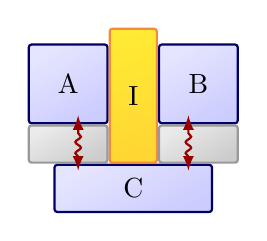
\begin{tikzpicture}
  \def\dl{0.027}
  \draw[bath]
    (-0.3-\dl,1.5) rectangle ++(-1,-1) node[midway] {A};
  \draw[bath]
    ( 0.3+\dl,1.5) rectangle ++( 1,-1) node[midway] {B};
  \draw[bath]
    (-1,-\dl) rectangle ++(2,-0.6) node[midway] {C};
  \draw[insulator]
    (-0.3,0) rectangle ++(0.6,1.7) node[midway] {I};
  \draw[conductor]
    (-0.3-\dl,0) rectangle ++(-1,0.5-\dl);
  \draw[conductor]
    ( 0.3+\dl,0) rectangle ++(+1,0.5-\dl);
  \path[draw,<->,thick,mydarkred,
        decorate,decoration={snake,amplitude=1,segment length=4,pre length=5,post length=5}]
    (-0.7,-0.1) --++ (0,0.7);
  \draw[<->,thick,mydarkred,
        decorate,decoration={snake,amplitude=1,segment length=4,pre length=5,post length=5}]
    ( 0.7,-0.1) --++ (0,0.7);
\end{tikzpicture}

% 0th LAW
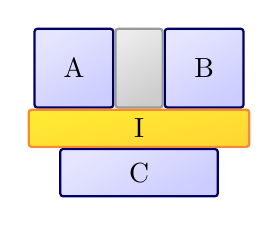
\begin{tikzpicture}
  \def\dl{0.027}
  \draw[bath]
    (-0.3-\dl,1.5) rectangle ++(-1,-1) node[midway] {A};
  \draw[bath]
    ( 0.3+\dl,1.5) rectangle ++( 1,-1) node[midway] {B};
  \draw[bath]
    (-1,-\dl) rectangle ++(2,-0.6) node[midway] {C};
  \draw[conductor]
    (-0.3,1.5) rectangle ++(0.6,-1);
  \draw[insulator]
    (-1.4,0) rectangle ++(2.8,0.5-\dl) node[midway] {I};
\end{tikzpicture}


% HEAT SOURCE & SINK
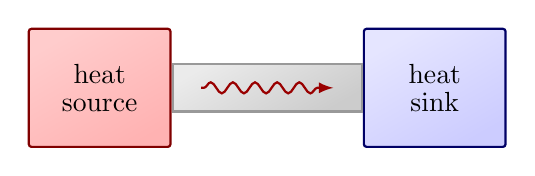
\begin{tikzpicture}[scale=1.5]
  \def\l{0.8}
  \def\dl{0.0185}
  \draw[source]
    (-\l-\dl,-0.5) rectangle ++(-1.2,1) node[midway,align=center] {heat\\[-2pt]source};
  \draw[bath]
    ( \l+\dl,-0.5) rectangle ++( 1.2,1) node[midway,align=center] {heat\\[-2pt]sink};
  \draw[conductor,rounded corners=0]
    (-\l,-0.2) rectangle ++(2*\l,0.4);
  \draw[->,thick,mydarkred,
        decorate,decoration={snake,amplitude=2,segment length=8,pre length=1,post length=5}]
    (-0.7*\l,0) --++ (1.4*\l,0);
\end{tikzpicture}


% SERIAL
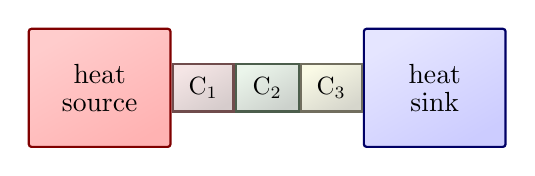
\begin{tikzpicture}[scale=1.5]
  \def\l{1.6}
  \def\dl{0.0185}
  \draw[source]
    (-\l/2-\dl,-0.5) rectangle ++(-1.2,1) node[midway,align=center] {heat\\[-2pt]source};
  \draw[bath]
    ( \l/2+\dl,-0.5) rectangle ++( 1.2,1) node[midway,align=center] {heat\\[-2pt]sink};
  \draw[C1]
    (-\l/2,-0.2) rectangle ++(\l/3-\dl,0.4) node[midway,scale=0.9] {C$_1$};
  \draw[C2]
    (-\l/6,-0.2) rectangle ++(\l/3,0.4) node[midway,scale=0.9] {C$_2$};
  \draw[C3]
    (\l/6+\dl,-0.2) rectangle ++(\l/3-\dl,0.4) node[midway,scale=0.9] {C$_3$};
\end{tikzpicture}


% PARALLEL
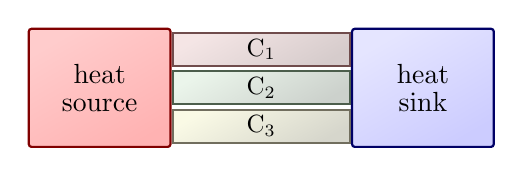
\begin{tikzpicture}[scale=1.5]
  \def\l{1.5}
  \def\dl{0.0185}
  \draw[source]
    (-\l/2-\dl,-0.5) rectangle ++(-1.2,1) node[midway,align=center] {heat\\[-2pt]source};
  \draw[bath]
    ( \l/2+\dl,-0.5) rectangle ++( 1.2,1) node[midway,align=center] {heat\\[-2pt]sink};
  \draw[C1]
    (-\l/2, 0.185) rectangle ++(\l,0.28) node[midway,scale=0.9] {C$_1$};
  \draw[C2]
    (-\l/2,-0.14) rectangle ++(\l,0.28) node[midway,scale=0.9] {C$_2$};
  \draw[C3]
    (-\l/2,-0.185) rectangle ++(\l,-0.28) node[midway,scale=0.9] {C$_3$};
\end{tikzpicture}


% PARALLEL
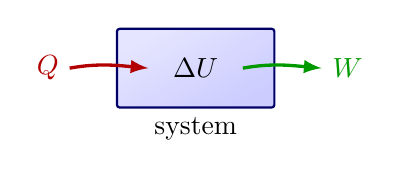
\begin{tikzpicture}[xscale=0.5,yscale=0.25]
  \draw[bath] (-2,-2) rectangle ++(4,4) node[midway,align=center,scale=1] {$\Delta U$};
  \node[below] at (0,-2) {system};
  \draw[<-,very thick,red!70!black]   (-1.2,0) to[out=170,in=20]++ (-2,0) node[left] {$Q$};
  \draw[->,very thick,green!60!black] ( 1.2,0) to[out=20,in=170]++ ( 2,0) node[right] {$W$};
\end{tikzpicture}


% HEAT SOURCE & SINK
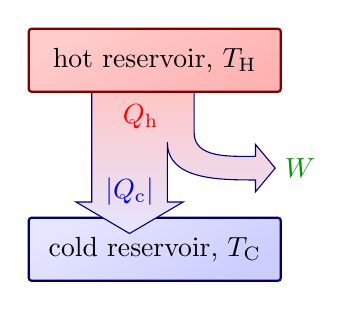
\begin{tikzpicture}
  \def\H{.8}
  \def\W{3.2}
  \def\L{1.6}
  \def\dl{0.0185}
  \coordinate (H) at (0, \L/2);
  \coordinate (C) at (0,-\L/2);
  
  \draw[bath]
    (C)++(-.4*\W,0) rectangle ++(\W,-\H) node[midway,align=center] {cold reservoir, $T_\text{C}$};
  
  \draw[mydarkblue,top color=red!22,bottom color=blue!10]
    (H) ++ (-.15*\W,0) -- (-.15*\W,.2-\L/2) --++ (-.2,0) --
    (0,-.2-\L/2) -- (.2+.15*\W,.2-\L/2) --++ (-.2,0) -- % large arrow: cold reservoir
    (.15*\W,.1*\L) to[out=-90,in=180] (.5*\W,-.2*\L) --++
    (0,-.15) --++ (.25,.3) coordinate (W) --++ (-.25,.3) --++ (0,-.15) % small arrow: work
    to[out=180,in=-90] (.5+.1*\W,.2+.05*\L) -- (.5+.1*\W,\L/2);
  
  \draw[source]
    (H)++(-.4*\W,0) rectangle ++(\W,\H) node[midway,align=center] {hot reservoir, $T_\text{H}$};
  
  \node[red,right=4,below=1] at (H) {$Q_\text{h}$};
  \node[mydarkgreen,right=0] at (W) {$W$};
  \node[blue,above=1] at (C) {$\abs{Q_\text{c}}$};
  
\end{tikzpicture}


% REFRIGERATOR
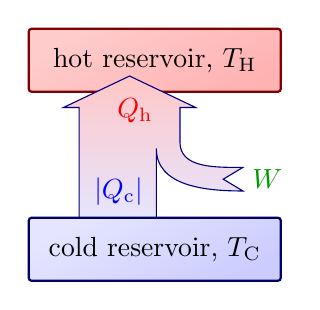
\begin{tikzpicture}
  \def\H{.8}
  \def\W{3.2}
  \def\L{1.6}
  \def\dl{0.0185}
  \coordinate (H) at (0, \L/2);
  \coordinate (C) at (0,-\L/2);
  
  \draw[source]
    (H)++(-.4*\W,0) rectangle ++(\W,\H) node[midway,align=center] {hot reservoir, $T_\text{H}$};
  
  \draw[mydarkblue,top color=red!22,bottom color=blue!10]
    (C) ++ (-.2*\W,0) -- (-.2*\W,-.2+\L/2) --++ (-.2,0) --
    (0,.2+\L/2) -- (.2+.2*\W,-.2+\L/2) --++ (-.2,0) -- % large arrow: cold reservoir
    (.2*\W,.1*\L) to[out=-90,in=180] (.45*\W,-.1*\L) --++
    (-0.25,-0.15) coordinate (W) --++ (0.25,-0.15) % small arrow: work
    to[out=180,in=-90] (.2*\W-0.3,.05*\L) -- (.2*\W-0.3,-\L/2);
    
%    (.15*\W,.1*\L) to[out=-90,in=180] (.5*\W,-.2*\L) --++
%    (-.25,.17) coordinate (W) --++ (.25,.17) % small arrow: work
%    to[out=180,in=-90] (.5+.1*\W,.2+.05*\L) -- (.5+.1*\W,\L/2);
  
  \draw[bath]
    (C)++(-.4*\W,0) rectangle ++(\W,-\H) node[midway,align=center] {cold reservoir, $T_\text{C}$};
  
  \node[red,right=2,below=-1] at (H) {$Q_\text{h}$};
  \node[mydarkgreen,right=7] at (W) {$W$};
  \node[blue,left=4,above=1] at (C) {$\abs{Q_\text{c}}$};
  
\end{tikzpicture}


\end{document}
